\subsection{分析方法概述}
对于数据集的分析,本文主要采用了EDA(Exploratory Data Analysis)的思想。\\
EDA是一种采用各种方法(主要指数据迹线、直方图、概率图等图形化方法)的数据分析方法。EDA的优势主要包括:
\begin{itemize}
	\item 最大限度地洞察数据集
	\item 揭示底层结构
	\item 提取重要变量
	\item 检测异常值
	\item 测试基本假设
	\item 建立初步模型
	\item 确定最佳因子设置
\end{itemize}
本章初步分析了题目数据集,了解数据集特征的同时也完成了传统的数据清洗、特征工程环节。便于后续和本文提出的新模型进行分析对比。
\subsection{具体分析}
通过查看好坏比、缺失值、相关度矩阵,初步确定数据集存在不平衡、缺失值和噪声等,需要清洗。
本节挑选具有代表性的属性进行分析。其他属性采用类似的分析方法,故不赘述。
\subsubsection{Age}
\begin{itemize}
	\item 查看数据分布情况
	      \begin{figure}[H]
		      \centering
		      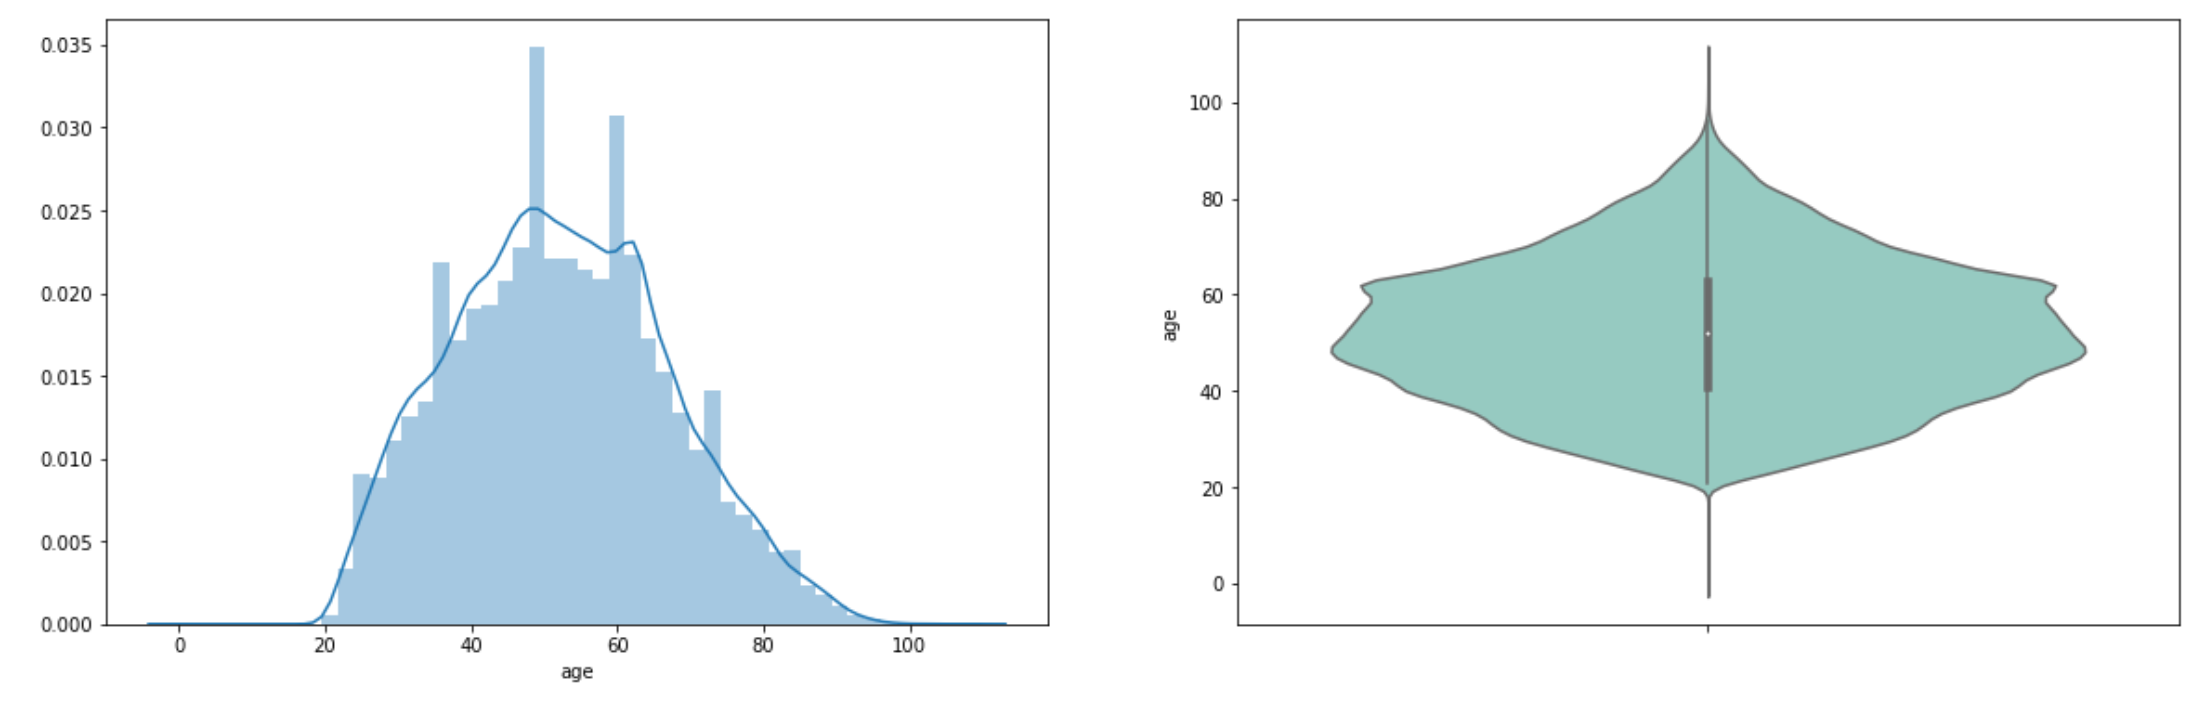
\includegraphics[width=1.0\linewidth]{age_distribution.png}
		      \caption{Age的分布情况}
	      \end{figure}
	      可见数据大致符合正态分布,存在一定噪声。同时由于年龄属性的特殊性,后续的数据清洗工作中需要估计年龄的上下界,以便更好消噪。
	\item 利用直方图查看age和预测值间的关系
	      \begin{figure}[H]
		      \centering
		      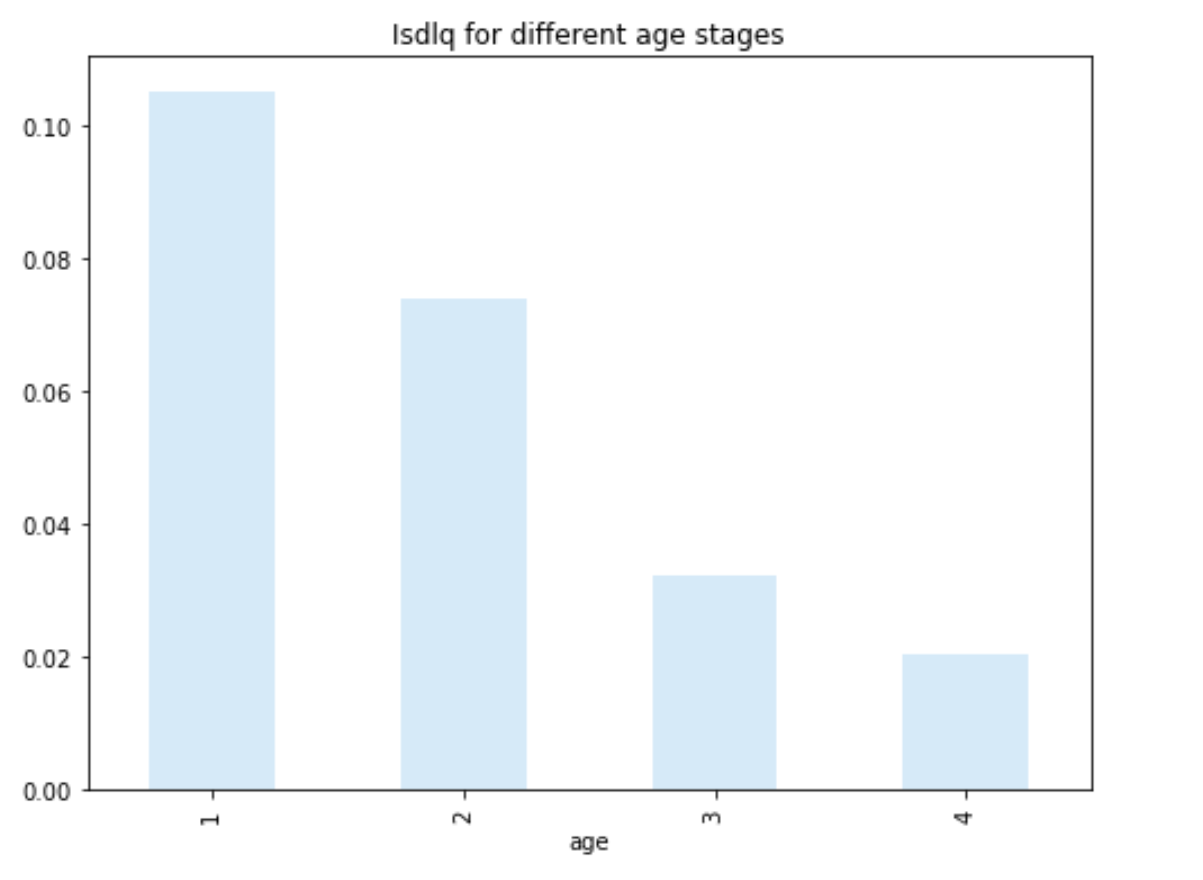
\includegraphics[width=0.8\linewidth]{age_histogram.png}
		      \caption{Age和Isdlq的关系}
	      \end{figure}
	      可见违约率随年龄递减。
	      \subsubsection{Revol}
	\item 查看数据分布情况
	      \begin{figure}[H]
		      \centering
		      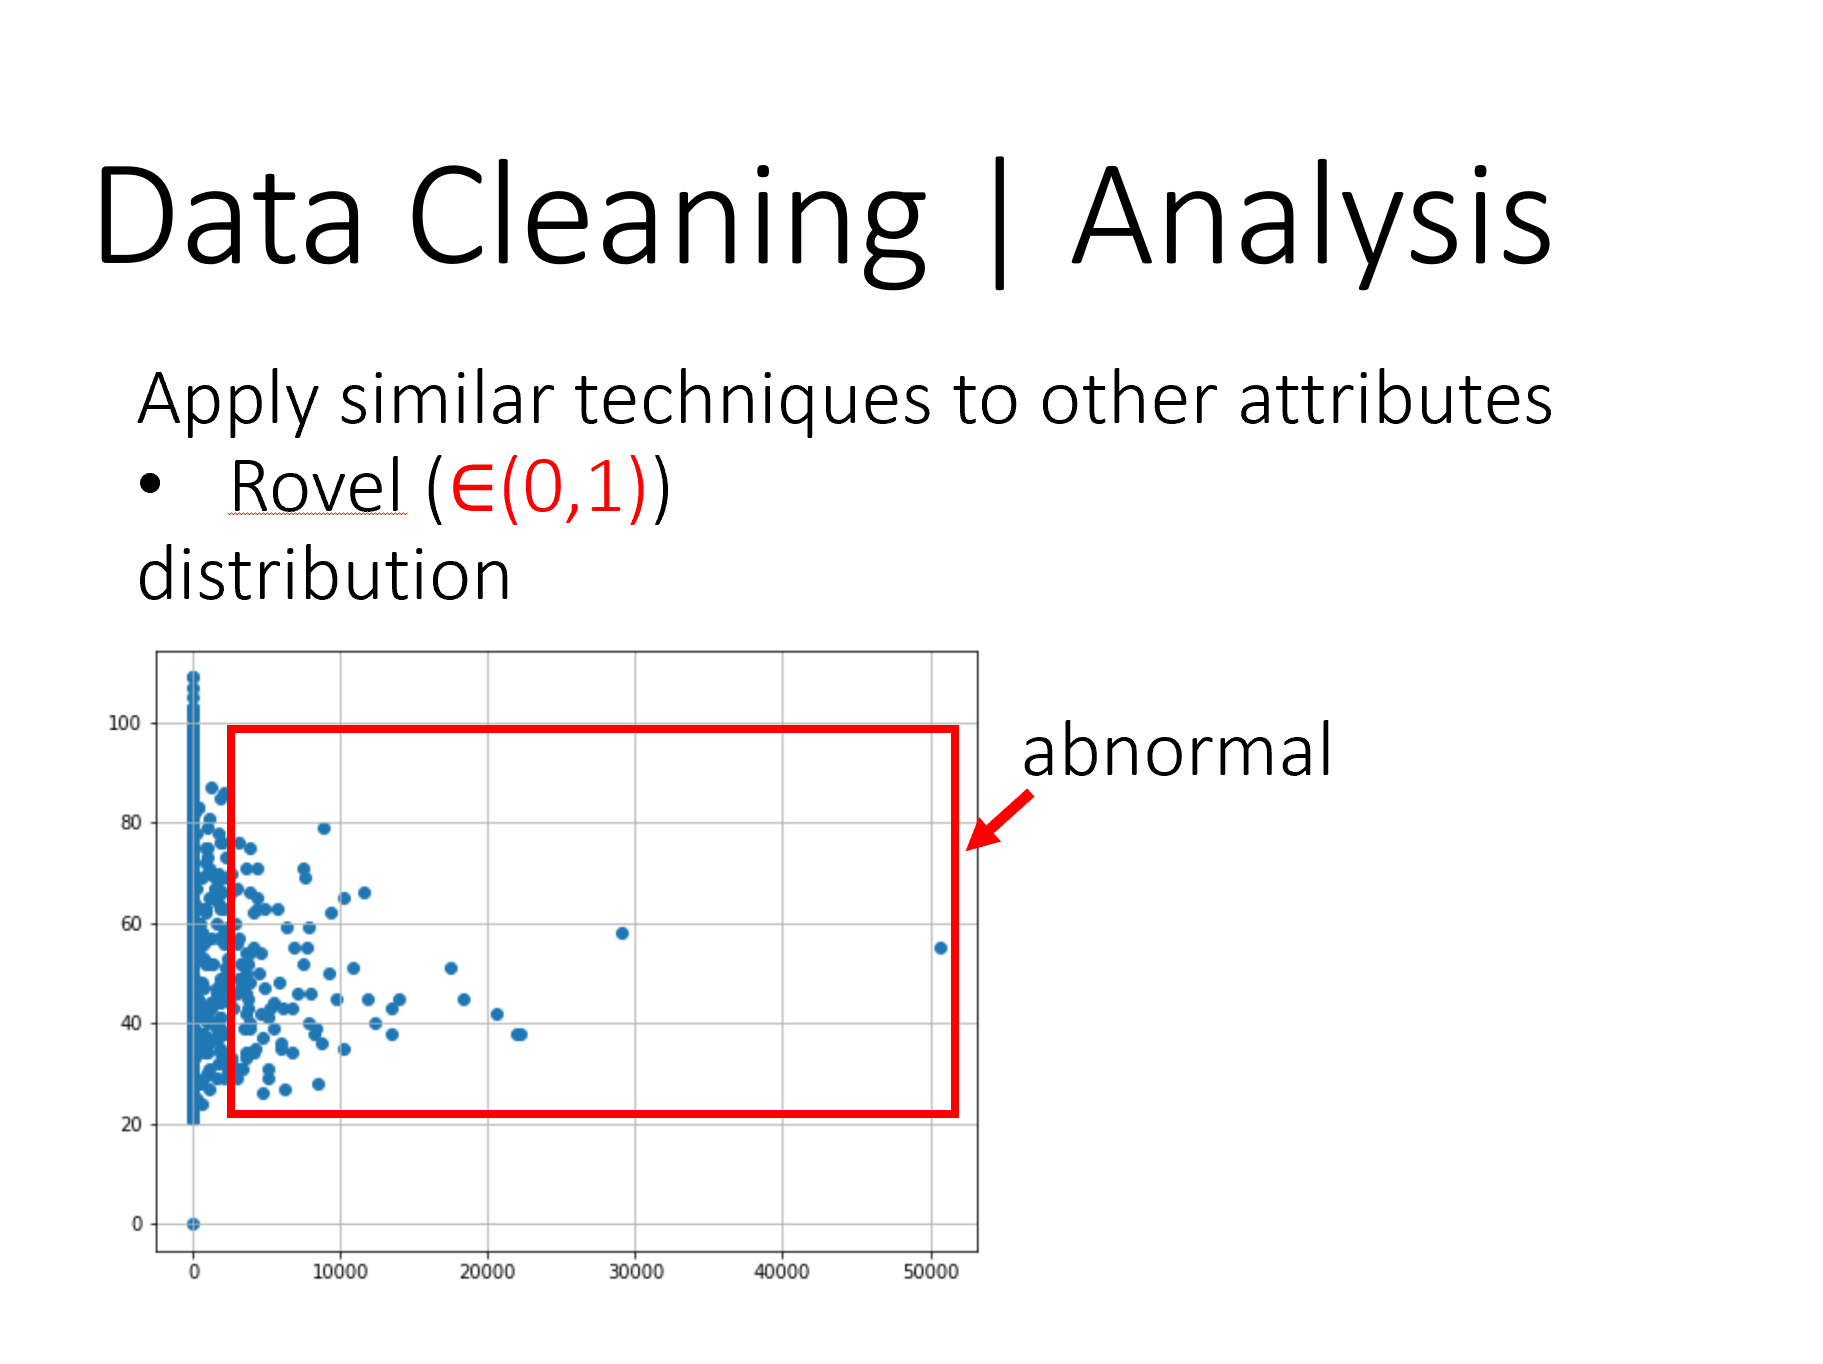
\includegraphics[width=0.6\linewidth]{revol_distribution.png}
		      \caption{Revol的分布情况}
		      \label{fig:rd}
	      \end{figure}
	      值得注意的是,Revol的合理区间应该是[0,1],而数据中却出现了明显的异常值。异常值可能来自于噪声,也可能来自于未规约化的正常数据。为了更大程度利用数据,本文继续查看了不同scale的数据直方图,大致确定可以舍去的异常值的范围。
	\item 利用不同scale直方图估计异常值区间
	      \begin{figure}[H]
		      \centering
		      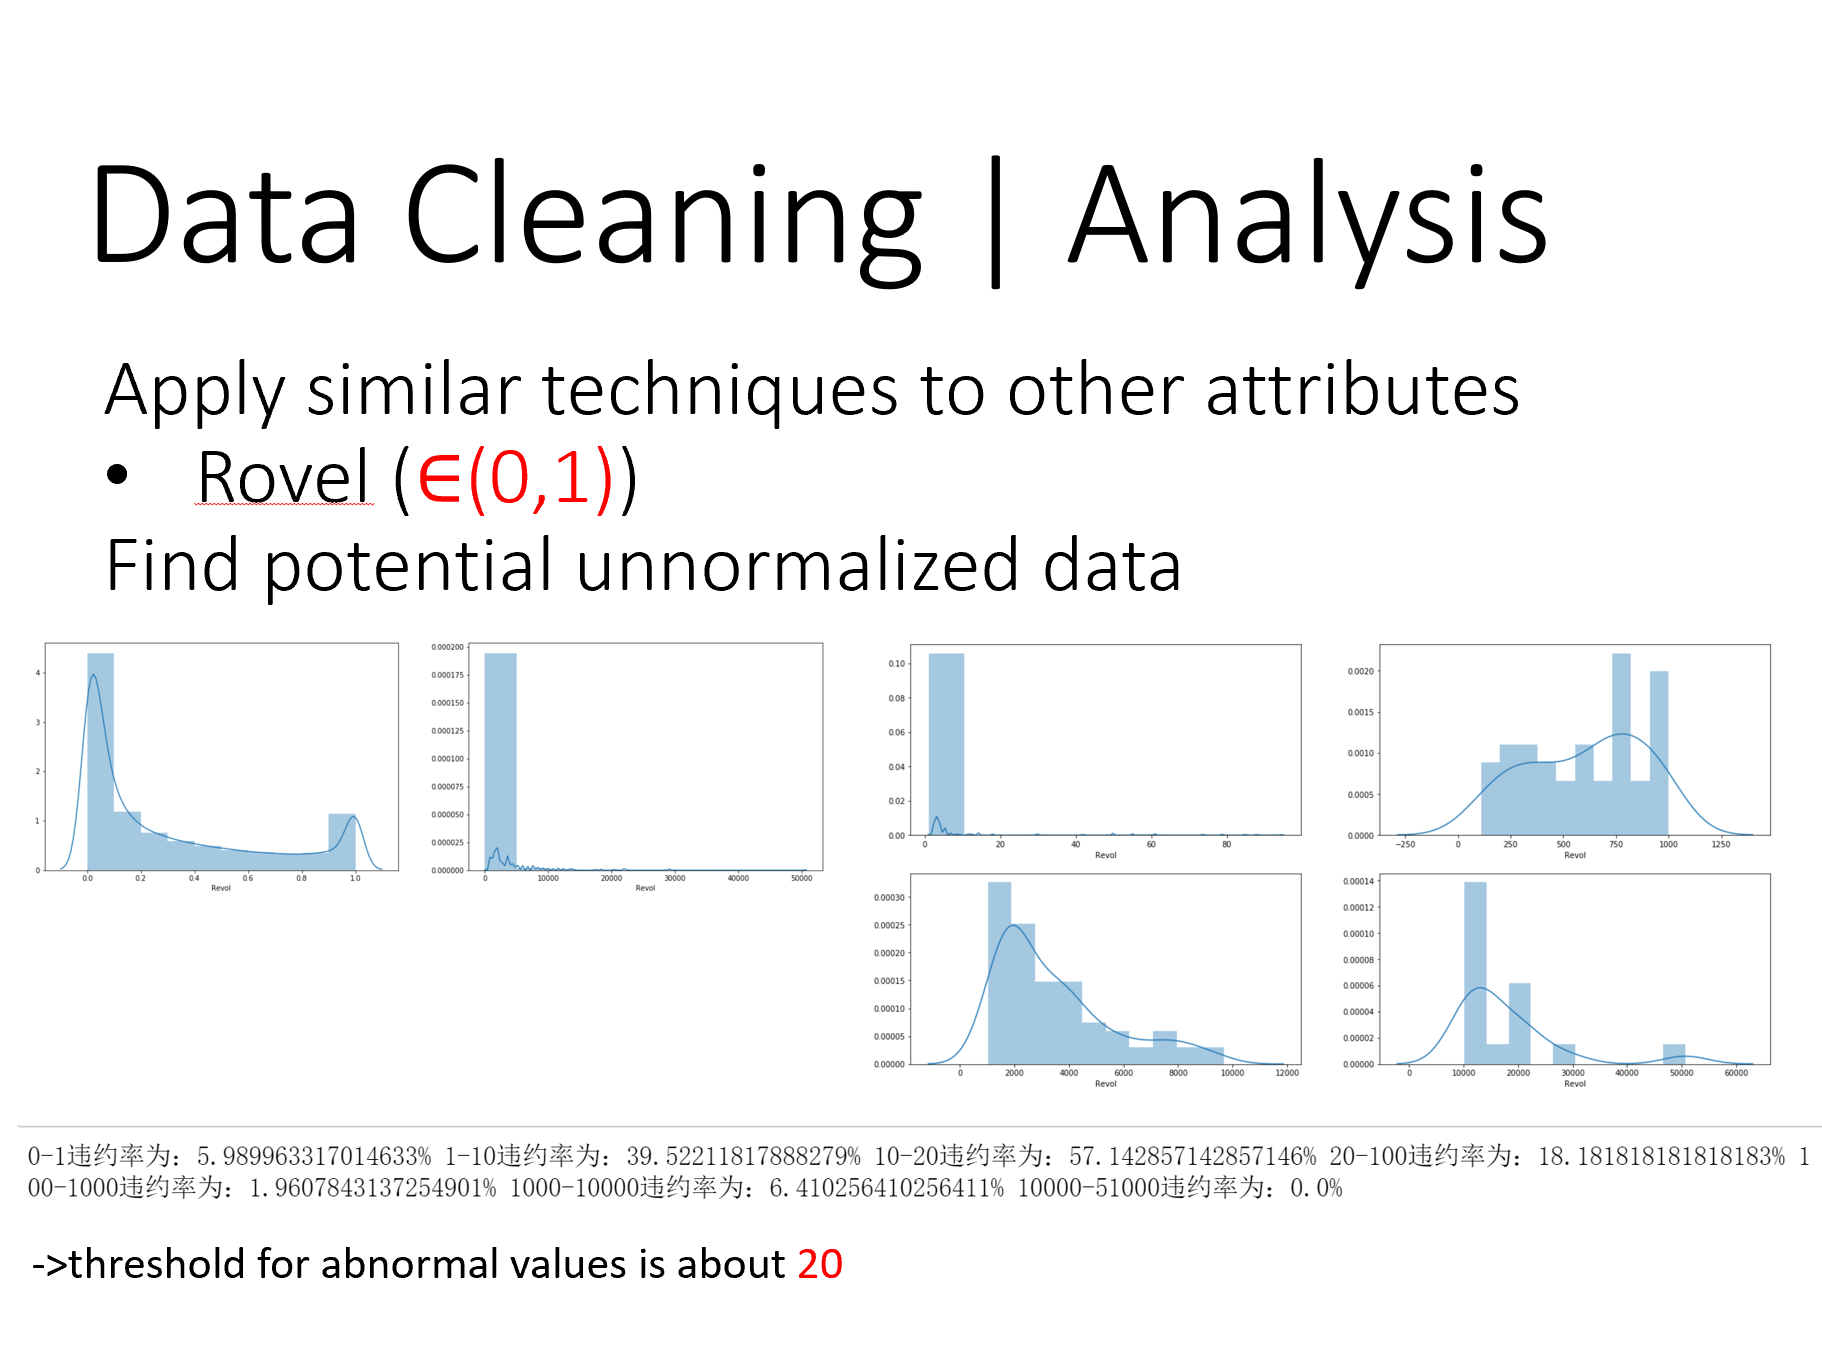
\includegraphics[width=0.8\linewidth]{revol_find_bounds.png}
		      \caption{不同区间的Revol直方图}
		      \label{fig:rh}
	      \end{figure}
	      因数据分布跨度比较大,我们将数据分为两部分,小于1和大于1的部分。\\
	      可以看出在Revol大于1时,违约率开始上升,10-20之间违约率达到高峰,超过20后开始下降,超过1000后开始恢复正常(与0-1的违约率一致),说明20左右的值可能为异常值上限的阈值。可以将超过20的值都定义为异常值。     
\end{itemize}

\subsection{数据清洗}
根据EDA分析中得出的结论。对数据集进行清洗,本文采用的具体方法包括异常值处理,缺失值填补,特征交叉衍生,数据类型转换、分箱等。
\begin{figure}[H]
	\centering
	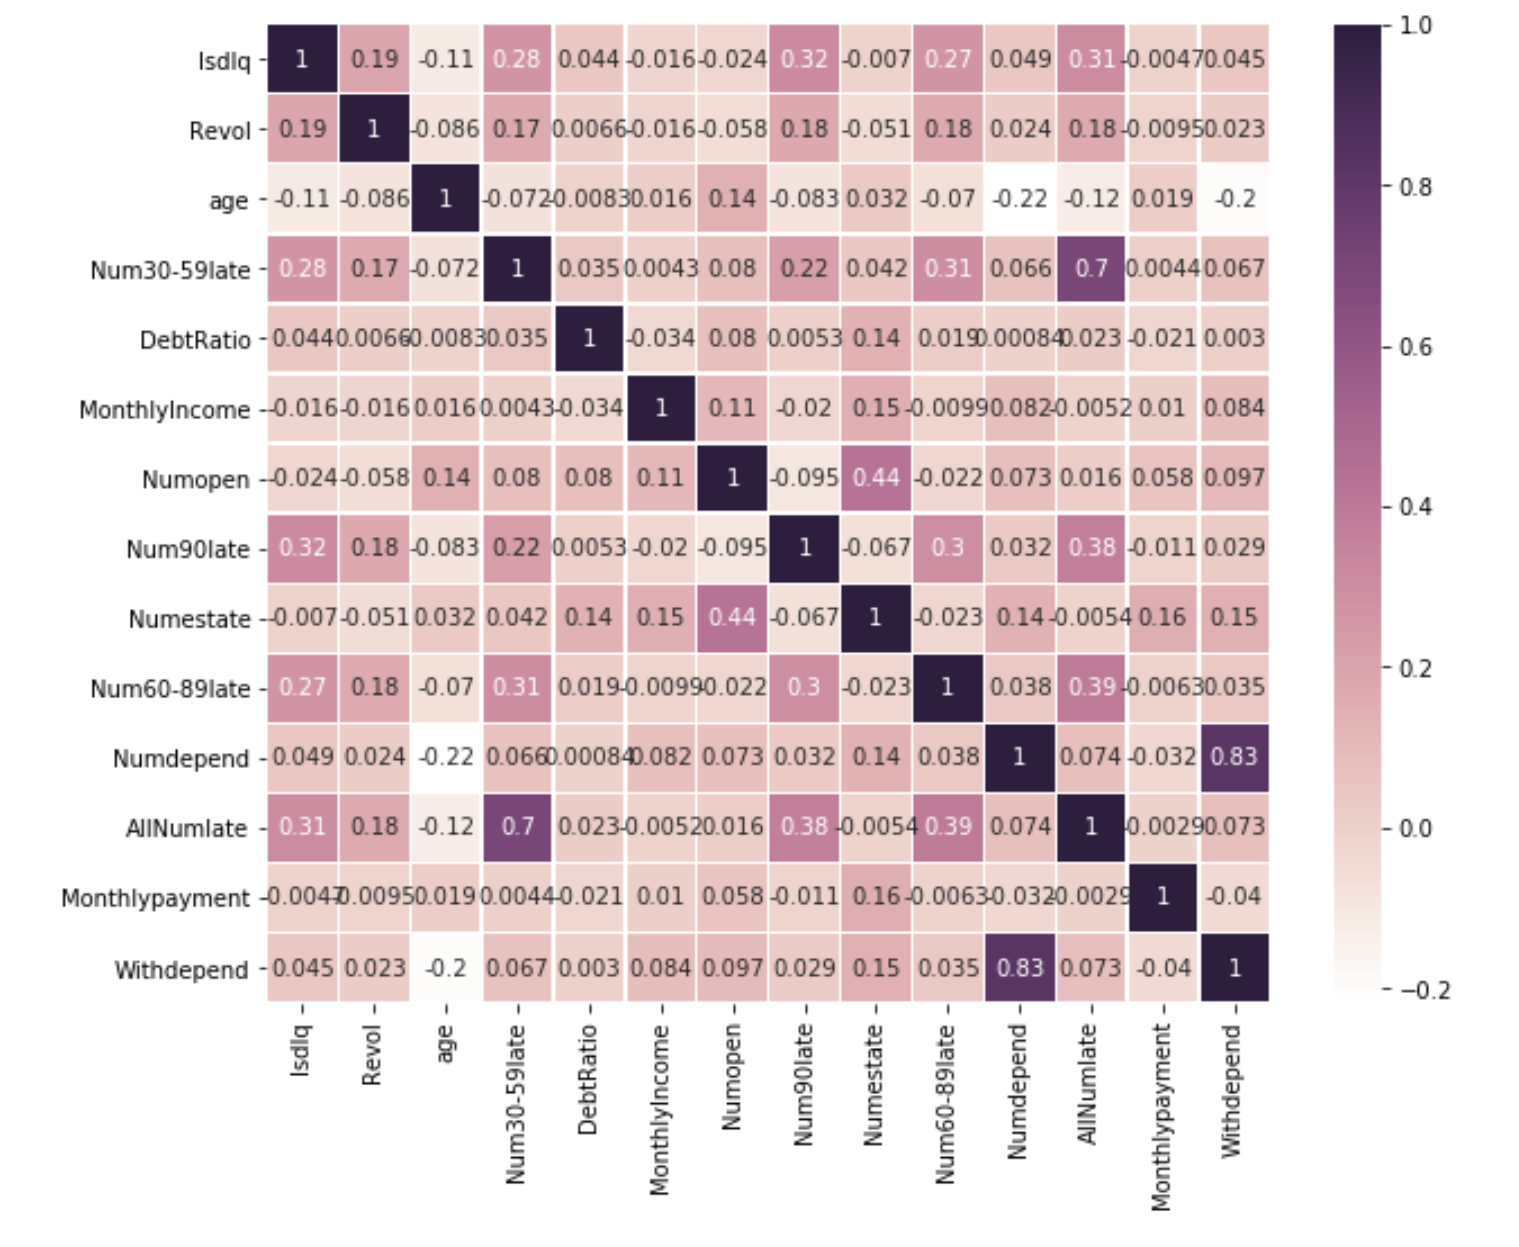
\includegraphics[width=0.9\linewidth]{heatmap.png}
	\caption{初步清洗后的相关度矩阵热力图}
	\label{fig:hm}
\end{figure}
其中,相关系数绝对值和两个变量关联程度成正比。

\subsection{特征筛选}
计算每个属性的WOE、IV值,如下图所示:
\begin{figure}[H]
	\centering
	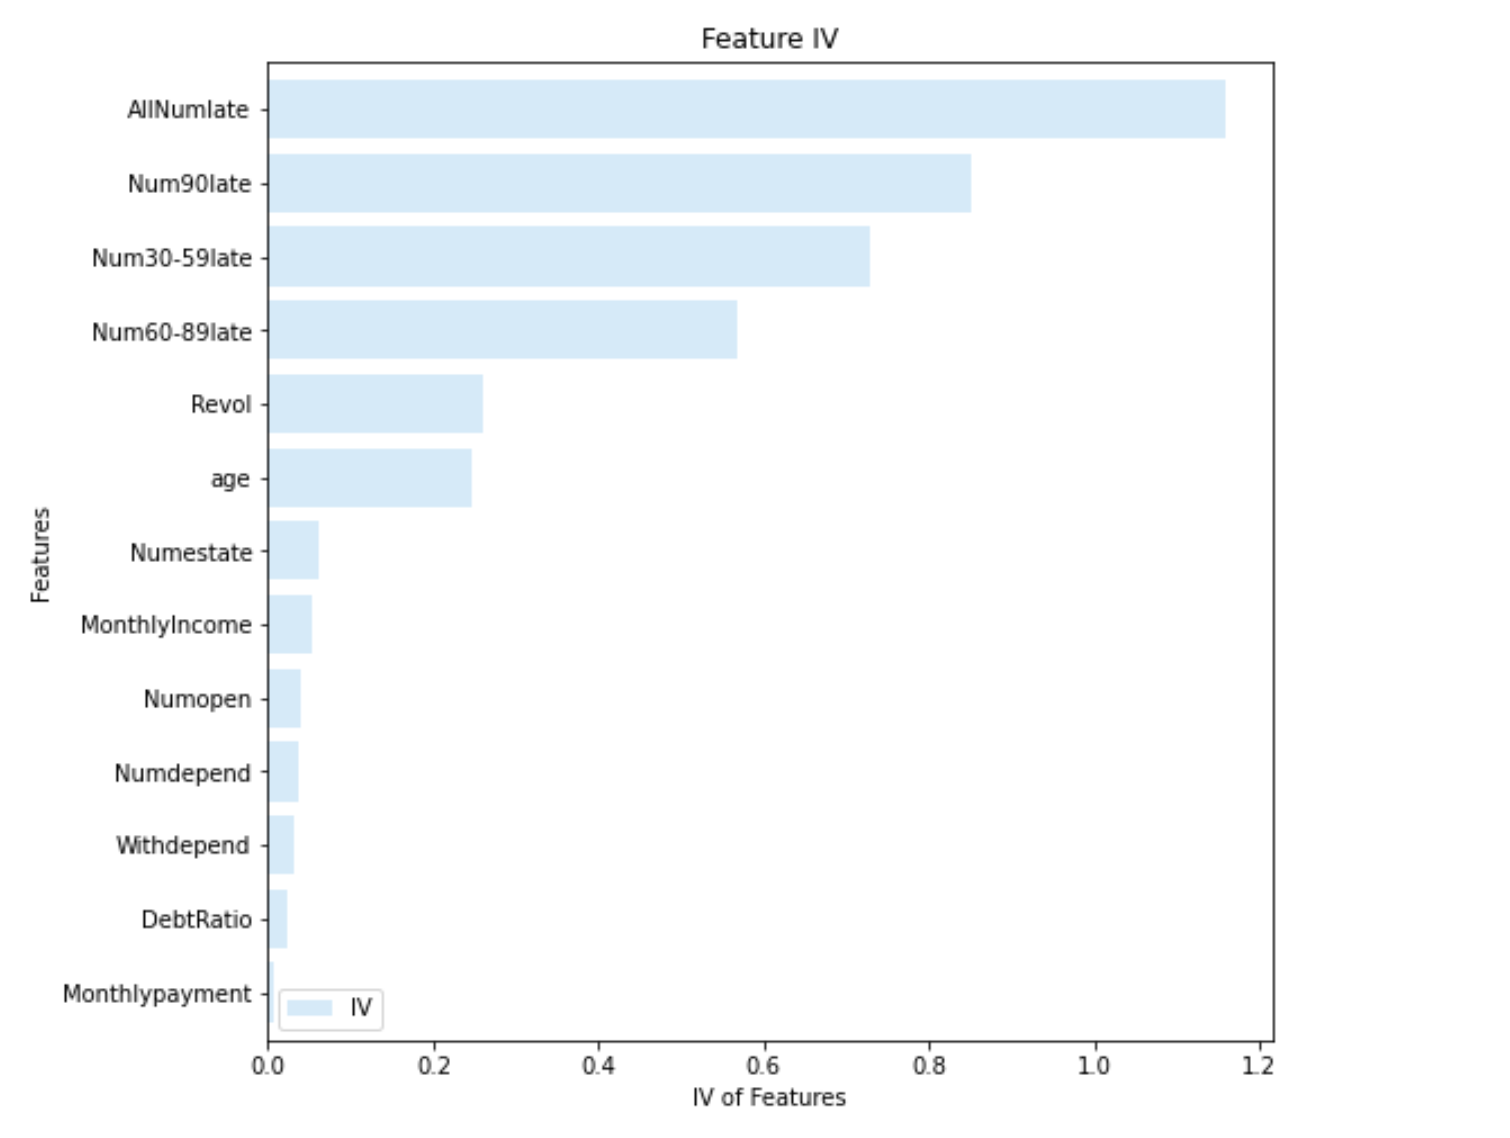
\includegraphics[width=0.8\linewidth]{IV.png}
	\caption{各属性IV值}
	\label{fig:iv}
\end{figure}

首先筛选出IV值大于0.1的变量:'Num30-59late','Num60-89late','Num90late','AllNumlate','Revol','age'。\\

从热力图看出,'Num30-59late'与'AllNumlate'具有强相关性(0.7),说明两者表征的信息具有较大的重叠,可以删掉一个。最终,两者取IV值较高者'AllNumlate'。
清洗后,最终选用特征 ['Num60-89late','Num90late','AllNumlate','Revol','age']。





